\documentclass[a4paper]{ctexart}
\usepackage{ctex}
\usepackage{xcolor}
\pagestyle{plain}
\usepackage{geometry}
\geometry{left=3.0cm, right=3.0cm, top=2.0cm, bottom=2.0cm}
\usepackage{graphics}
\usepackage{hyperref}
\usepackage[nounderscore]{syntax}
\AtBeginDocument{\catcode`\_=8 }
\usepackage{minted}
\usepackage{makecell}
\usepackage{listings}
\usepackage{amssymb}
\usepackage{amsmath}
\newenvironment{typewriterfont}{\ttfamily}{\par}
\ctexset{section/format = {\Large\bfseries}}
\hypersetup{
colorlinks=true,
linkcolor=black
}

\begin{document}

\begin{titlepage}
    \mbox{}
    \vskip 8 cm
    \centering

    \Huge 编译实习课程改革\ 实习报告
    \rule{\textwidth}{1pt}\par % Thick horizontal line

    \huge 李汪洋\ 李佳蔚\ 梁家硕

    \Large \today

\end{titlepage}
\tableofcontents
\newpage

\section{编译实习课程}

\subsection{编译课程概览}

目前北京大学的编译原理(编译技术)课程与编译实习课程,是形式上独立而实际上紧密结合的两门课程。编译原理主要讲授理论,编译实习主要动手实践。

编译原理课程前半学期主要讲:正则表达式与自动机、词法分析、上下文无关的语法分析、语法制导翻译。后半学期主要讲:中间代码生成、运行时环境、寄存器分配、代码优化。

编译实习课程的任务是实现一个MiniJava的编译器,以巩固编译原理课程上学到的知识。总体流程是:MiniJava $\rightarrow$ Piglet $\rightarrow$ Spiglet $\rightarrow$ Kanga $\rightarrow$ MIPS。

\subsection{MiniJava任务的一些缺陷}

由于课程内容设计和选课系统的一些原因,还无法将这两门课合并成一门课,而且两门课程在进度上有些不协调。由于编译原理与编译实习两课程联系紧密,同学们通常在同一学期同时选修这两门课程。根据之前同学们的反映,两门课经常出现进度差异问题,比如实习课要用到的技术在原理课上还没有讲,实习课前半学期基本只做前端工作导致后半学期工作量过大等等。

MiniJava任务是同学单人完成,同学们可能头一次面对这样的大项目,做起来可能有些吃力。但对于一些能力较强的同学,也可能觉得任务有些简单。

在MiniJava编译器整体任务由词法分析、语法分析、寄存器分配等多个小任务组成,小任务间环环相扣,同学们如果在之前的某一环没有完成好,可能影响之后代码编写和完成进度。

另外,编译课程不要求先修Java程序设计,而MiniJava虽然语法不复杂,但其编译器要求用Java实现,对于没有接触过Java的同学有些不友好。

\subsection{课程改革}

我们设计出一套全新的MiniC编译器框架,以替代当前编译实习课程使用的MiniJava,来解决编译课程目前面临的一系列问题。并希望能与信息科学技术学院的体系结构实习、操作系统实习等课程的改革结合,帮助学生更好地理解计算机科学与技术。

编译实习课程改革的目标主要有三点。

一,在一定程度上降低门槛,让能力不太强的同学也能顺利完成任务,体验编译器的编写流程,对于能力较强的同学,提供一些可选的扩展内容。

二,尽可能配合编译原理课程进度,更合理地进行任务分配。

三,使任务模块化,单独对某一阶段知识点进行实践测试,对于先前已经做完的任务,提供标准模块,避免项目前面遗留问题对后期进度的影响。

\newpage
\section{MiniC编译器}

\subsection{概述}

MiniC编译器的目标是把MiniC语言一步一步转化成合法的32位RISC-V汇编。

MiniC编译器,除了MiniC语言外,还涉及Eeyore和Tigger两种中间语言,和最终要输出的RISC-V汇编。

MiniC编译器总共有3个必要大步骤,总体流程是:MiniC $\rightarrow$ Eeyore $\rightarrow$ Tigger $\rightarrow$ RISC-V。

MiniC, Eeyore, Tigger的设计都遵循简洁易读的原则,方便同学处理。同学们没必要使用Eeyore或Tigger的全部语法,如果觉得使用它们的某个子集就能完成任务也是可以的。%(其实我们认为Eeyore和Tigger已经高度精简,没必要再取子集了)

Eeyore和Tigger这两个名称,继承了MiniJava编译器中使用到的Piglet和Kanga的命名传统。都取自同一动画``Winnie Pooh"。

\begin{center}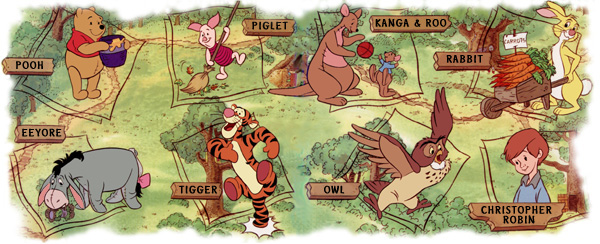
\includegraphics[width=15cm]{name} \end{center}

据了解,以往同学们MiniJava编译器编写时遇到的困难主要有三点:课程进度问题、类型检查复杂琐碎、寄存器分配算法有难度。我们的解决方案分别是,重新安排课程进度使之与原理课程匹配,减少数据类型的数量,推荐一些更好写的寄存器分配算法(相比原理课上讲的图染色法)。

\subsection{MiniC}

MiniC是C语言的一个子集,我们对C语言进行了大量的删减,力图产生一种高度精简的、易于实现的语言。对于MiniC的语言定义与描述,参考附录中的“MiniC说明”。

MiniC编译器的第一步,是实现MiniC语言的词法分析和语法分析(可以利用lex和yacc等工具),并分析语义,将MiniC转换成Eeyore中间语言。

MiniC的类型只有int和一维int数组,极大地减小了类型检查的工作量。

\subsection{Eeyore}

Eeyore是一中三地址码,为了让同学们易于接受,Eeyore的语法是编译原理课程教学用书(龙书)中使用的三地址码格式的扩展。具体描述参考附录中的“Eeyore说明”。

Eeyore可以看作是MiniC编译器中的Piglet和Spiglet。

在这一步,要做的是优化(可选)和寄存器分配工作。输入Eeyore代码,输出Tigger格式的中间代码。

\subsection{* 优化}

优化阶段不是必须的,有能力的同学可以选做。在考核方面,可单独对产出的Eeyore的运行速度进行测试。

编译优化阶段的输入和输出格式都是Eeyore。

\subsection{Tigger}

Tigger可以被认为是Eeyore进行了寄存器分配后的版本,与Eeyore语法很像。具体描述参考附录中“Tigger说明”。

Tigger可以看作是MiniC编译器中的Kanga。

在这一步,要做的是把Tigger代码转换为RISC-V汇编。这几乎是一句对应一句的简单文本处理了。

\subsection{RISC-V}

生成合法的RISC-V汇编之后,同学们要做的所有工作就完成了。

我们会调用riscv-gcc把生成的RISC-V汇编转成机器码。

最终使用RISC-V的模拟器运行机器码,并进行最终的整体测试。(中间步骤的完成情况使用我们编写的Eeyore和Tigger模拟器进行阶段性测试)

\subsection{进度安排}

根据我们小组完成各阶段所用的时间,我们对同学们的MiniC编译器任务做了如下初步进度安排。(我们小组的完成进度在下一节)

第1--2周:努力学习编译原理,并预习语法制导翻译部分,并尝试学习安装riscv-gcc。

第3--7周:完成MiniC$\rightarrow$Eeyore。具体地说,第3周实现符号表与类型检查,第4周完成词法分析,第5周完成文法书写,第6周处理表达式翻译,第7周处理控制流翻译。

第8--11周:完成Eeyore$\rightarrow$Tigger。具体地说,第8周完成Eeyore的语法树构建,第9周实现活性分析,第10周实现寄存器分配,第11周输出Tigger代码。

第12--13周:完成Tigger$\rightarrow$RISC-V。包括熟悉RISC-V汇编和输入输出格式处理。

第14周:编写实验报告。

可以看出,以上时间安排没有占满整个学期的时间,这是考虑到同学们有期中期末考试以及假期,预留出了2周左右的时间。根据我们自己的经验,主要的难度在于Eeyore和Tigger的产生,而最后一步相对比较容易,所以还可以有一周时间用于活动安排或者用于扩展内容或程序优化。

\newpage
\section{工作完成情况}

\subsection{MiniC方面}
\begin{itemize}
	\item 完成MiniC语法制定
	\item 完成MiniC的parser
\end{itemize}

前半学期花了很多时间实现了复杂MiniC语法的parser,几乎是把所有扩展内容都实现了。

parser使用on-the-f\/ly翻译模式,维护了一个极复杂但表达能力很强的符号表,如果只是翻译base语法集可以删去很多没必要的类型与检查。

parser编写过程中遇到了C语言中不区分布尔表达式与其他表达式的问题,这会使原理课上学的回填技术无法使用。为了解决这个问题parser放弃了回填技术,但仍用on-the-f\/ly翻译模式,只是先计算表达式的值,然后再进行逻辑判断。这样做使得遇到逻辑表达式时产出的代码略冗长,但确实解决了问题,也能正确处理\texttt{||}与\texttt{\&\&}短路跳转。为了让同学们方便处理,base语法集限定布尔表达式不可以是算术表达式。

另外,C语言的文法(用lex和yacc表示的)可以直接从网上找到,我们希望同学们能自己完成MiniC文法的编写,不要直接抄网上现成的lex和yacc代码。

\subsection{Eeyore方面}

\begin{itemize}
	\item 完成Eeyore语法制定
	\item 完成Eeyore模拟器
	\item 完成Eeyore上的寄存器分配算法,把Eeyore转化成Tigger
\end{itemize}

即使是在已经简化过的 Eeyore 文法上,也是较为复杂一步。预处理使用了 lex + yacc,建出符号表。寄存器分配使用了 Linear Scan 算法,相较于之前的 web + 图染色算法,大大简化。

这步比较麻烦的是在最后生成 Tigger 代码的时候,会有许多特殊情况。寄存器与变量之间的关系较为混乱,稍有不慎就会写错。另一个难点是处理数组,这里需要对数组,地址等概念非常清晰。

处理种种特殊情况时,为了代码实现的更简明一些,在某些细节上会产生一些浪费现象。处理这些细节也是一个有技术难度的工作,可以考虑作为扩展内容。

关于 Linear Scan 算法的详细说明,详见 Linear Scan 的说明文档。

\subsection{Tigger方面}

\begin{itemize}
	\item  完成Tigger语法制定
	\item  完成Tigger模拟器
	\item  完成Tigger转为RICS-V汇编
\end{itemize}

Tigger模拟器的实现,先利用lex和yacc构建语法树(其实基本是一条链),在运行之前给全局变量赋值,然后从\texttt{f\_main}开始执行,执行过程中维护栈和寄存器的值。

由于Tigger语法很简单,模拟器实现起来没什么困难。

Tigger模拟器同Eeyore模拟器一样,也实现了调试功能,帮助同学们调试寄存器分配算法。
\\

\subsection{评测方面}
\begin{itemize}
	\item 完成测试平台搭建
	\item 完成测试程序以及测试数据构造
\end{itemize}

测试程序都是些MiniC程序,这些程序有大有小,可以比较全面地对编译器的正确性和产出代码的质量进行测试。但是因为我们对编译测试的原理不太熟悉,所以测试程序可能设计的有一些缺陷,这一点我们可以之后进一步修正。

对于每个MiniC测试程序,我们都构造了一些测试数据,每个测试数据包括一个输入文件和一个答案文件。

我们没有专门构造Eeyore和Tigger的测试集,因为同学们有可能不会用到Eeyore和Tigger的全部语法。因此,Eeyore和Tigger的测试程序应由MiniC的测试程序经过转化而来,测试数据与之前的相同。

评测平台我们使用的是CMU开源的Autolab测试平台,也就是我们学校著名的ICS课程使用的测试平台,实现在线测评和统计成绩。

\subsection{计划与现实}

说实话,没想到选编译实习课程改革这个题目会有这么大的任务量,时间很紧张。虽然每个小任务的不太难,但任务数量很多。

按照开题时的计划,期中前基本要把完整的编译器做出来,期中后实现一些工具和测试脚本,设置扩展内容。

事实上,在期中前,我们用了大量时间设计了一套比现在看到的复杂得多的MiniC和三地址码,并完成实现了它们的parser和模拟器。

中期报告后紧接着的一两周,小组三人都忙于各种考试与其他任务,没时间写代码。在老师与助教的指点下,意识到同学们不太可能实现这么复杂的语法,就在这段时间制定了一套从头到尾全新的MiniC,Eeyore,Tigger语法,明确了之后要做的工作。

现在看来,在期中前我们相当于实现了大部分扩展内容,体验了一把复杂的扩展内容是多么难写。

最后的几周,完成的工作比较多。为提供运行效率重写了Eeyore模拟器。为了减轻同学们的负担,也为了小组能尽快完成任务,学习并实现了Linear Scan寄存器分配算法。编写了Tigger模拟器。测试程序和测试数据集,搭建了测试平台。

\newpage
\section{写给后来人}

在实践过程中,我们深切体会到课程改革之不易。我们的工作也许只是改革的一个开端,想真正投入教学,还需实践检验。我们在这里记录下编译实习课程改革的一些经验,希望能对之后投身这项课程改革的人们有些许启发。
\\

Eeyore模拟器和Tigger模拟器可作为测试工具提供给同学,完成的MiniC编译器的三大步骤的代码,可以用作标准模块。

如果不使用标准模块,同学们可以只使用Eeyore和Tigger语言的一个子集,把自己产出的那个子集翻译好就可以正确地产生RISC-V代码了。如果同学在前面的某个步骤没能顺利完成,那么把标准模块提供给他时,他可能会面临标准模块产出的代码超出了他原本使用的那个子集这样的问题。

我们小组只保证标准模块之间能正确拼接成一个正确的编译器,同学们写的模块与标准模块拼接时可能会出现不兼容的问题,因为我们目前手上只有自己写的标准模块,还无法做这方面的测试工作。
\\

MiniC语法扩展内容,也许无法被翻译成Eeyore或Tigger代码,这是因为Eeyore和Tigger是专门为MiniC的base语法集制定的,无法表达一些base以外的语法。所以对于想做MiniC语法扩展内容的同学,只能对扩展内容单独测试,同学们要想办法把扩展的部分最终转成RISC-V,比如可以自行扩展Eeyore和Tigger的语法使它们支持扩展内容。
\\

同学们若想本地测试自己生成的RISC-V汇编是否正确,需要先下载并编译riscv-tools,再利用riscv-gcc生成机器码,最后用RISC-V的模拟器来运行。在我们小组编译riscv-tools的过程中,遇到了大量奇怪的编译错误,RISC-V官方并没有给出多少对于这些编译错误的说明,致使我们花费了不少时间来解决这些错误。我想同学们在尝试编译riscv-tools的时候,也许会觉得很头大。

\newpage
\section{收获}

\noindent 李佳蔚:

第一个收获是把之前编译技术没学明白的东西都彻底搞明白了。编译实习这门课的特点就是如果不彻底搞明白原理,根本没法写代码。发明Eeyore和Tigger语法的过程也对自己的能力有很大提高。发明一种语言比使用一种语言,对理解的要求高得多。

第二个收获是积累了很多与一个小团队一起合作写工程的经验。这是我第一次写比较大的工程,所以在这期间学到了许多写工程的基本常识和技巧,这种能力的提高在将来发展中也一定会有很大帮助。

第三个也是最大的收获就是完成了一件富有现实意义的工作。真心希望该项目能作为课程改革的一个起点,最终惠及广大信科师生。

\bigskip
\noindent 梁家硕:

巩固了编译技术课程上学到的知识,一些看起来不难的算法,其实实现起来细节很多,必须亲身实践才能透彻领悟。

小组合作使我深切体会到团队的力量。项目的任务量比较大,团队的协作与沟通给了我很大的鼓舞,两位队友的表现很出色,让我有信心能把自己的任务完成。

从前对汇编几乎一窍不通,该项目的工作使我头一次接触到RISC-V汇编,也许对今后的学习有所帮助。

参与教学改革、提高教学质量,大概之前做梦也想不到会做这样的项目吧。当了一回课程设计者,不仅对该课程有了更多的理解,也对“教育”与“学习”本身的有了不同于从前的认识。

\bigskip
\noindent 李汪洋:
两位小同学代码能力很强,我只是实力打酱油,总的来说算是把四大礼包选完了,也算是把去年体系课学到的一些东西用上了,学会了使用Lex/Yacc来写东西,感觉还是蛮有意思的。

项目大体上是做完了,但是还有一些细节的东西应该还要完善,可能还需要后续维护一下。

\newpage
\section{附录}
以下内容是完整的MiniC、Eeyore、Tigger语法描述与定义。

三种语言都有各自的文档,内容与以下部分相同。三个分离的文档可提供给同学们,以便查阅。
\subsection{MiniC说明}
\subsubsection{概述}
MiniC是C语言的一个子集,对C语言语法进行了大量删减,以产生一种适用于编译实习课程的语言。

MiniC是为了取代原先编译实习课程使用的MiniJava语言而设计的,目的是更好地配合编译原理课程进度,在一定程度上减轻任务量。MiniC基础语法%(我们称之为base语法集)
高度精炼,使同学们无论能力如何,都能完成编译器编写的过程。

同时,对于能力较强的同学,实习课程可以提供一些MiniC语法扩展内容,把从C语言中删除的一些语法加回MiniC,来提升MiniC语言的易用程度和表达能力,对完成扩展内容的同学提供一定程度的加分。

\subsubsection{语法描述}
\begin{itemize}
\item 
MiniC取消了C语言中的宏。%即取消了编译预处理过程。
\item 
MiniC中的变量有两种类型,int和一维int数组。%(没有void类型,没有指针)
\item
MiniC中函数返回值只有int,参数可以是int或int数组,程序从main函数开始执行。同时,MiniC不会给函数默认返回值,如果执行完一个函数而没有return,会导致未知行为。

%另外,MiniC中的函数都有return语句,即使返回值无意义,也要以return一个数的方式结束函数。
\item 
单目运算符有\texttt{'!'}和\texttt{'-'}
\item
双目运算符有\texttt{'+','-','*','/','\%','\&\&','||','\textless','\textgreater','==','!='}
\item
合法的表达式参考BNF。
\item 
允许使用函数前置声明(参见样例中\texttt{getint}函数)。
\item 
MiniC程序中允许C风格的单行注释。%和多行注释。
\item 
MiniC只保留\texttt{if-else}条件分支语句和\texttt{while}循环语句。
\item 
为了使MiniC更容易实现,限定\texttt{if,while}后面的括号里和逻辑运算符两边的运算分量只会出现如下两种形式:\\
\indent\ \ \texttt{x>y||(a+b)!=c}这样的逻辑表达式;\\
\indent\ \ \texttt{x}或\texttt{f(x)}或\texttt{a[x]}这样的单个变量或函数。\\
\indent 总之,不会出现类似\texttt{if (a+b)}或\texttt{(b+c)||d}这样的语句。
\end{itemize}
\newpage
\subsubsection{BNF}
\setlength{\grammarindent}{8em} % increase separation between LHS/RHS 
\begin{typewriterfont}
\begin{grammar}
<Goal> ::= (VarDefn | FuncDefn | FuncDecl)* MainFunc

<VarDefn> ::= Type Identifier ';'
\alt Type Identifier'['<INTEGER>']' ';'

<VarDecl> ::= Type Identifier
\alt Type Identifier'['<INTEGER>?']'

<FuncDefn>  ::= Type Identifier '(' ( VarDecl ( ',' VarDecl )* )? ')' '\{' (FuncDecl | Statement)* '\}'

<FuncDecl> ::= Type Identifier '(' ( VarDecl (',' VarDecl)*)?')' ';'

<MainFunc> ::= 'int' 'main' '(' ')' '\{' (FuncDecl | Statement)* '\}'

<Type> ::= 'int'

<Statement> ::= '\{' (Statement)* '\}'
\alt 'if' '(' Expression ')' Statement ('else' Statement)?
\alt 'while' '(' Expression ')' Statement
\alt Identifier '=' Expression ';'
\alt Identifier '[' Expression ']' '=' Expression ';'
\alt VarDefn
\alt 'return' Expression ';'

<Expression>	::=	Expression ( '+' | '-' | '*' | '/' | '\%' ) Expression
\alt Expression ( '\&\&' | '||' | '\textless' | '==' | '\textgreater' | '!=' ) Expression
\alt Expression '[' Expression ']'
\alt <INTEGER>
\alt Identifier
\alt ( '!' | '-' ) Expression
\alt Identifier '(' (Identifier (',' Identifier)*)? ')'
\alt '(' Expression ')'

<Identifier>	::=	<IDENTIFIER>

\end{grammar}
\end{typewriterfont}

\newpage
\subsubsection{示例}
\small
\begin{minted}[linenos]{c}
int getint(); // 前置函数声明,getint函数是MiniC内置函数,返回一个读入的整数
int putchar(int c); // 内置函数,用于输出字符(参数为ascii码),返回值无意义
                    // 注意!base语法集不包括形如int putchar(int);这种参数名没有具体给出的函数声明
int putint(int i); // 内置函数,用于输出整数,返回值无意义
int getchar(); // 内置函数,返回一个读入的字符的ascii码 (此程序未使用到该函数)
int f(int x) /* 该函数以递归方式计算Fibonacci数 */
{
    if (x < 2) /* if-else语句 */
        return 1;
    else
        return f(x - 1) + f(x - 2); /* 递归函数调用 */
}
int g(int x) /* 该函数以数组和循环语句计算Fibonacci数 */
{
    int a[40]; /* int数组声明
                  注意!base中数组大小必须是常数,不可写成int a[x];或int a[10+30];这样*/
    a[0] = a[1] = 1;
    int i;
    i = 2; /* 注意!base语法集不包括初始化赋值语句  int i = 2; */
    while (i < x + 1) /* while循环是base语法集唯一的循环语句 */
    {
        a[i] = a[i - 1] + a[i - 2];
        ++i;
    }
    return a[x];
}
int n; // 声明了一个全局变量
int main() {
    n = getint();
    if (n < 0 || n > 30) /* 不带else的if语句 */
        return 1;
    putint(f(n));
    putchar(10); // 输出换行符
    putint(g(n));
    putchar(10);
    return 0;
}
\end{minted}
\newpage
\normalsize
\subsubsection{MiniC语法扩展}
MiniC设计者们亲身实践了MiniC大部分语法扩展,深切体会到实现一些复杂语法扩展的不宜。

对MiniC语法进行扩展时,应尽量遵循“细致”的原则,避免涉及范围过大的扩展。

比如,整数数据类型扩展:加入8位,16位,32位,64位的有符号和无符号整数。这个扩展涉及的范围就有些大,可以考虑分解成多个扩展:带符号整数扩展、不同长度的整数运算扩展、char字符串扩展(8位有符号整数组成的数组)、字符与字符串表示扩展(加入\texttt{"abc",'\textbackslash n'}这样的表达式)。

具体可以扩展内容,按教学通知为准。

\newpage
\definecolor{bg}{rgb}{0.85,0.85,0.85}
\subsection{Eeyore说明}
\subsubsection{概述}
Eeyore /\texttt{'}\i:ju\textschwa(r)/ 是一种三地址码,用作MiniC语法分析后的输出格式。Eeyore的设计同样遵循简洁的原则,使代码易读易调试。

%Eeyore在MiniC编译器中的地位,对应着MiniJava编译器中使用到的Piglet和SPiglet两种中间语言。

%Eeyore这个名字与Piglet取自同一部动画。

\subsubsection{语法描述}
Eeyore要求\textbf{每条语句单独占一行}。

\noindent \textbf{变量}
\begin{itemize}
\item 
Eeyore中的变量有三种:原生变量,临时变量,函数参数。这三种变量分别以\texttt{'T','t','p'}开头,后接一个整数编号,编号从0开始,每个函数单独编号。如\texttt{p0,p1,t0,T0}。

\item 
Eeyore的变量声明形如\texttt{var t0}和\texttt{var 8 T0},前者声明了一个int型临时变量,后者声明了有2个元素的原生int数组。

\item
\textbf{注意!函数参数不需要声明。}

\item 
除函数参数变量外,其余变量不允许重名。

\item 
函数内声明的变量作用域为变量声明语句到函数结束语句,函数外声明的变量作用域为变量声明语句到程序最后。

\item 
所谓原生变量,是指MiniC中使用的变量转到Eeyore中对应的变量。相应地,临时变量是指MiniC中没有显式对应变量的变量。

\qquad 其实这两种变量在语义上\textbf{没必要做如此区分},Eeyore区分二者是为了方便用户调试。用个例子来说明,把左边的MiniC语句翻译到Eeyore:
\begin{table}[H]
    \centering
    \small
    \begin{typewriterfont}
    \begin{tabular}{|c|c|}
        \hline
        MiniC & Eeyore \\
        \hline
        \makecell[l]{int a;\\ int b;\\ int c;\\a = b + 2 * c;} & \makecell[l]{var T0\\var T1\\var T2\\var t0\\t0 = 2 * T2\\var t1\\t1 = T1 + t0\\T0 = t1} \\
        \hline
    \end{tabular}
    \end{typewriterfont}
\end{table}

上面\texttt{T0,T1,T2}是原生变量,分别对应MiniC中的\texttt{a,b,c}。\texttt{t0,t1}是临时变量,分别对应中间运算结果\texttt{2*c, b+2*c}。

\end{itemize}
\noindent \textbf{表达式}
%由上面的例子可以发现,Eeyore的表达式很易读。

%因为是三地址码,每条表达式语句最多涉及三个变量。

Eeyore表达式有以下特点:
\begin{itemize}

\item 
允许直接把整数用作运算分(如\texttt{t0 = 2 * T2})。

\item
Eeyore表达式支持的单目运算符有\texttt{'!','-'}

\item 
支持的双目运算符有\texttt{'!=','==','\textgreater'.'\textless','\&\&','||','+','-','*','/','\%'},前6个是逻辑运算符。

\item 
数组操作语句形如\texttt{T0 [t0] = t1}和\texttt{t0 = T0 [t1]}。

\item
注意!因为MiniC的base语法集只有int和int数组类型,数组操作语句中括号内的数应当是4的倍数。

%注意!如果\texttt{T0}是数组,那\texttt{t0 = T0 + 4}这样的语句实际上是指针运算,\texttt{t0}的类型是int不是数组。
\end{itemize}
\noindent \textbf{函数}
\begin{itemize}
\item 
Eeyore中的函数以\texttt{'f\_'}开头,后接函数名,如\texttt{f\_main,f\_getint}。

\item 
函数定义语句形如\texttt{f\_putint [1]},中括号内的整数表示该函数的参数个数,函数结束处应有函数结束语句,形如\texttt{end f\_xxx}。

\item 
函数外的变量声明语句被视为全局变量声明,函数内的视为局部变量声明。

%函数调用语句形如\texttt{t0 = call f\_xxx}。如果该函数有参数,还需要在调用语句前插入传参语句,形如\texttt{param t1},每个传参语句只传一个参数,如有多个参数,应按照参数顺序一个一个传。
\item 
函数调用语句形如: \texttt{t0 = call f\_xxx}。

\item 
传参数指令形如: \texttt{param t1},所有传参都是\textbf{传值},多个参数需依次传入。

\item
作为参数的变量,在\texttt{param Variable}语句之后,到函数调用前,不可修改。(这样限制的目的是使寄存器分配时避免繁琐的分类讨论)

\item
函数返回语句形如\texttt{return t0}。
\end{itemize}
\noindent \textbf{标号与跳转}
\begin{itemize}
\item 
Eeyore中的标号以小写字母\texttt{'l'}开头,后接整数编号,编号从0开始,如\texttt{l0,l1}。标号用来指明跳转语句的跳转地点,标号声明语句形如\texttt{l0:}。

\item
跳转语句分两种:无条件跳转、条件跳转。如\texttt{goto l1}和\texttt{if t0 < 1 goto l0}。

%不允许跨函数跳转。
\end{itemize}
\noindent \textbf{缩进}

Eeyore没有缩进要求,但是允许缩进,为了之后代码调试的便利,我们建议正确使用缩进。

\noindent \textbf{注释}

Eeyore允许单行注释,与C语言注释类似使用\texttt{//},处理时自动忽略改行从\texttt{//}之后所有内容。

\noindent \textbf{系统库支持}

Eeyore模拟器提供对输入输出的系统调用支持,对应的函数原型如下:
\begin{itemize}
	\item \texttt{int getint()} //从标准输入读取一个整数
	\item \texttt{int putint(int x)} //输出x到标准输出
	\item \texttt{int getchar()} //从标准输入中读取一个字符
	\item \texttt{int putchar(int x)} //输出ASCII为x的字符
\end{itemize}
具体对应的MiniC代码和Eeyore代码用法参见章节“\textbf{示例}”
\newpage
\subsubsection{BNF}
\begin{typewriterfont}
\setlength{\grammarindent}{8em} % increase separation between LHS/RHS 
\begin{grammar}
<Declaration> ::= 'var' <INTEGER>? Variable

<FunctionDecl> ::= Function '[' <INTEGER> ']' '\textbackslash n' ((Expression | Declaration)'\textbackslash n')* 'end' Function
%t1 = t1 <op>/<relop> t2
%t1 = <op> t2
%t1 = <type> t2 (类型转换)
%t1 = t2
%t1 [ t2 ] = t3
%* t1 = t2
%t1 = t2 [ t3 ]

<RightValue> ::= Variable | <INTEGER>

<Expression>	::=	Variable '=' RightValue OP2 RightValue
\alt Variable '=' OP1 RightValue
\alt Variable '=' RightValue
\alt Variable '[' RightValue ']' = RightValue
\alt Variable = Variable '[' RightValue ']'
\alt 'if' RightValue LogicalOP RightValue 'goto' Label
\alt 'goto' Label
\alt Label ':'
\alt 'param' RightValue
\alt Variable '=' 'call' Function
\alt 'return' RightValue


<Identifier>	::=	<IDENTIFIER>

<Variable> ::= <VARIABLE>

<Label> ::= <LABEL>

<Function> ::= <FUNCTION>

\end{grammar}
\end{typewriterfont}
\newpage
\subsubsection{示例}
\begin{table}[H]
    \centering
    \begin{typewriterfont}
    \begin{tabular}{|c|c|}
        \hline
        MiniC & Eeyore \\
        \hline
        \makecell[l]{
int getint();\\
int putint(int x);\\
int n;\\
int a[10];\\
int main()\\
\{\\
\ \ n = getint();\\
\ \ if (n > 10)\\
\ \ \ \ return 1;\\
\ \ int s;\\
\ \ int i;\\
\ \ i = 0;\\
\ \ s = i;\\
\ \ while (i < n) \{\\
\ \ \ \ a[i] = getint();\\
\ \ \ \ s = s + a[i];\\
\ \ \ \ ++i;\\
\ \ \}\\
\ \ putint(s);\\
\ \ return 0;\\
\}
        } & \makecell[l]{
var T0\\
var 40 T1\\
f\_main [0]\\
\ \ T0 = call f\_getint\\
\ \ var t0\\
\ \ t0 = T0 - 10\\
\ \ var t1\\
\ \ t1 = t0 > 0\\
\ \ if t1 == 0 goto l0\\
\ \ return 1\\
l0:\\
\ \ var T2\\
\ \ var T3\\
\ \ T3 = 0\\
\ \ T2 = T3\\
l1:\\
\ \ var t2\\
\ \ t2 = T3 < T0\\
\ \ if t2 == 0 goto l2\\
\ \ var t3\\
\ \ t3 = 4 * T3\\
\ \ var t4\\
\ \ t4 = call f\_getint\\
\ \ T1 [t3] = t4\\
\ \ var t5\\
\ \ t5 = T1 [t3]\\
\ \ T2 = T2 + t5\\
\ \ T3 = T3 + 1\\
l2:\\
\ \ param T2\\
\ \ call f\_putint\\
\ \ return 0\\
end f\_main
} \\
        \hline
    \end{tabular}
    \end{typewriterfont}
\end{table}

\newpage
\subsubsection{Eeyore模拟器使用方式}
\begin{typewriterfont}
\begin{lstlisting}
Usage ./Eeyore [-d] <filename>

-d : enable debug mode

- e.g. ./Eeyore -d test.in

出现"> "提示符表示进入debug模式,支持如下指令: 

+ p <pc/symbol/label/funciton name>     
    - e.g. p pc, p c1, p t1
    - Print the value of the symbol
+ s <number>
    - e.g. s 10
    - Run n Step
+ n
    - e.g. n
    - Run 1 Step
+ u <number/function/label>
    - e.g. u 10, u f_g, u l1
    - Run until pc equal to number or until the function or label.
+ r
    - e.g. r
    - Disable the debug mode and run until the program exit.
\end{lstlisting}
\end{typewriterfont}

\newpage
\subsection{Tigger说明}
\subsubsection{概述}
Tigger /\texttt{'}t\i g\textschwa (r)/ 是面向RISC-V的一种中间表示,用作寄存器分配的输出格式。

为了让同学们快速熟悉Tigger语法,Tigger遵循一贯的简洁易读风格,被设计得与Eeyore很像。

%Tigger在MiniC编译器中的地位,对应着MiniJava编译器中使用到的Kanga中间语言。

%Tigger这个名字与Kanga取自同一部动画。

\subsubsection{语法描述}

\noindent \textbf{寄存器}

Tigger共有28个可用的寄存器,这些寄存器的名称与RISC-V保持一致(相比RISC-V,删去了一些不需要编译器管理寄存器)。
\begin{itemize}
\item
\texttt{x0}:该寄存器恒等于0,不可更改

\item
\texttt{s0-s11}:没什么特殊之处,被调用者保存。

\item
\texttt{t0-t6}:没什么特殊之处,调用者保存。

\item
\texttt{a0-a7}:用来传递函数参数,调用者保存。其中a0-a1也被用作传递函数返回值,但因为MiniC中所有函数返回值都是int,所以实际上只有a0被用作传递返回值。
\end{itemize}
可以看出,最多只能通过寄存器传递8个参数。简单起见,限定所有函数参数个数不超过8个。

\noindent \textbf{表达式、标号、跳转语句}
\begin{itemize}
\item
所有的表达式计算都在寄存器上进行。

\item
所有在Eeyore中支持的运算符,在Tigger中都支持。

\item
注意!因为MiniC里只有int和int数组类型,所以形似数组赋值语句的赋值语句中括号内的数是4的倍数。

\item
注意!由于RISC-V某些规则的原因,Tigger中只有的\texttt{'+'}和\texttt{'<'}运算符允许作为\texttt{Reg = Reg OP2 <INTEGER>}语句中的\texttt{OP2}。

\item
标号与跳转语句和Eeyore中的语法相同,标号是全局的。
\end{itemize}
\textbf{函数}
\begin{itemize}
\item
函数定义语句形如\texttt{f\_xxx [2] [3]},第一个中括号内是参数个数,第二个是该函数需要用到的栈空间的大小(除以4之后)。

\item
函数结束语句和Eeyore中的一样,形如\texttt{end f\_xxx}。

\item
函数必须以返回语句返回。返回值通过寄存器传递。

\item
函数调用语句形如\texttt{call f\_xxx}。
\end{itemize}
\textbf{栈内存操作}

程序运行时,每个被调用的函数都会维护一个连续的栈空间,大小为函数定义语句中的第二个参数。

局部变量都可以在栈中找到,因此Tigger中不再有局部变量了。

\begin{itemize}
\item
\texttt{store Reg <INTEGER>}语句中,\texttt{<INTEGER>}是一个小于函数定义语句第二个系数的非负整数。该语句会把寄存器\texttt{<Reg>}的值存入当前函数栈空间第\texttt{<INTEGER>}个位置。

\item
\texttt{load <INTEGER> Reg}语句中,\texttt{<INTEGER>}是一个小于函数定义语句第二个系数的非负整数。该语句会把当前函数栈空间第\texttt{<INTEGER>}个整数存入寄存器\texttt{<Reg>}

\item
\texttt{loadaddr <INTEGER> Reg}语句中,\texttt{<INTEGER>}是一个小于函数定义语句第二个系数的非负整数。该语句会把当前函数栈空间第\texttt{<INTEGER>}个位置的内存地址存到寄存器\texttt{<Reg>}。
\end{itemize}

举个例子,假设某个时刻函数调用关系是\texttt{main[0][3] -> f[0][4]},正在执行函数\texttt{f},假设此时的栈如下图所示:

\begin{center}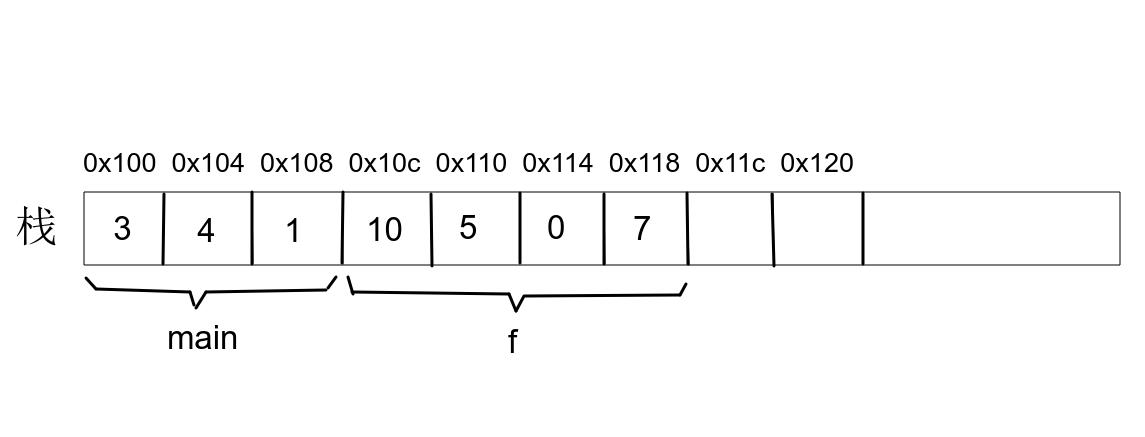
\includegraphics[height=4cm]{stack2}\end{center}

此时语句\texttt{load 2 s0},会使\texttt{s0 = 5};语句\texttt{loadaddr 2 s0},会使\texttt{s0 = 0x110};语句\texttt{store s0 2}会把图中的\texttt{5}改成\texttt{s0}的值。

\noindent \textbf{全局变量}

\begin{itemize}
\item
全局变量名称以\texttt{v}开头,后接一个整数编号,编号从0开始,比如\texttt{v0,v1}。

\item
\texttt{<VARIABLE> = <INTEGER>}用来声明一个初始值为\texttt{<INTEGER>}的全局变量\texttt{<VARIABLE>},即\texttt{<VARIABLE>}这个名称表示的内存地址上4字节的内容为\texttt{<INTEGER>}。

\item
\texttt{<VARIABLE> = malloc <INTEGER>}用来声明数组,\texttt{<VARIABLE>}这个名称表示的内存地址之后的\texttt{<INTEGER>}字节的内容为一个数组。
注意!\texttt{<INTEGER>}是4的倍数。

%对全局变量的操作都通过寄存器完成,全局变量的\texttt{load}和\texttt{store}语句与之前介绍的稍有不同。

\item
\texttt{load <VARIABLE> Reg}表示把\texttt{<VARIABLE>}这个全局变量对应内存地址上4字节的内容加载到寄存器\texttt{Reg}。

\item
\texttt{loadaddr <VARIABLE> Reg}表示把\texttt{<VARIABLE>}这个全局变量对应内存地址加载到寄存器\texttt{Reg}。

\item
注意!由于RISC-V汇编的原因,没有\texttt{store Reg <VARIABLE>}语句。该语句可以通过\texttt{loadaddr}语句与数组访问语句结合来完成。
\end{itemize}

\noindent \textbf{注释}

Tigger允许单行注释,与C语言注释类似使用//,处理时自动忽略改行从//之后所有内容。

\noindent \textbf{系统库支持}

与MiniC和Eeyore中的输入输出函数原型相同。

四种输入输出函数都通过\texttt{a0}寄存器传递参数和返回值。

\newpage
\subsubsection{BNF}
\setlength{\grammarindent}{8em} % increase separation between LHS/RHS 
\begin{typewriterfont}
\begin{grammar}
<Goal>  ::= (FunctionDecl | GlobalVarDecl)*

<GlobalVarDecl> ::= <VARIABLE> '=' <INTEGER>
\alt <VARIABLE> '=' 'malloc' <INTEGER>

<FunctionDecl> ::= Function '['<INTEGER>']' '['<INTERGER>']' (Expression)* 'end' Function

<Expression>	::=	Variable '=' Reg OP2 Reg
\alt Reg '=' Reg OP2 <INTEGER>
\alt Reg '=' OP1 Reg
\alt Reg '=' Reg
\alt Reg '=' <INTEGER>
\alt Reg '[' <INTEGER> ']' = Reg
\alt Reg = Reg '[' <INTEGER> ']'
\alt 'if' Reg LogicalOP Reg 'goto' Label
\alt 'goto' Label
\alt Label ':'
\alt 'call' Function
\alt 'store' Reg <INTEGER>
%\alt 'store' Reg <VARIABLE>
\alt 'load' <INTEGER> Reg
\alt 'load' <VARIABLE> Reg
\alt 'loadaddr' <INTEGER> Reg
\alt 'loadaddr' <VARIABLE> Reg
\alt 'return'

<Reg> ::= 'x0'
| 's0'
| 's1'
| 's2'
| 's3'
| 's4'
| 's5'
| 's6'
| 's7'
| 's8'
| 's9'
| 's10'
| 's11'
| 'a0'
| 'a1'
| 'a2'
| 'a3'
| 'a4'
| 'a5'
| 'a6'
| 'a7'
| 't0'
| 't1'
| 't2'
| 't3'
| 't4'
| 't5'
| 't6'

<Label> ::= <LABEL>

<Function> ::= <FUNCTION>

\end{grammar}
\end{typewriterfont}

\newpage
\subsubsection{示例}
\begin{typewriterfont}
\begin{lstlisting}
f_fac [1] [3]
    a0 = a0 + -1
    if a0 <= x0 goto l1
    store a0 0
    call f_fac
    store a0 1
    store s0 2
    loadaddr 0 s0
    a0 = s0[0]
    a0 = a0 + -1
    call f_fac
    a1 = s0[4]
    load 2 s0
    a0 = a0 + a1
    goto l2
l1:
    a0 = 1
l2:
    return
end f_fac

f_main [0] [0]
    call f_getint
    call f_fac
    call f_putint
    a0 = 10
    call f_putchar
    a0 = 0
    return
end f_main
\end{lstlisting}
\end{typewriterfont}

\newpage
\subsubsection{Tigger模拟器使用方式}
\begin{typewriterfont}
\begin{lstlisting}
Usage ./Tigger [-d] <filename>

-d : enable debug mode

- e.g. ./Tigger -d test.in

出现"> "提示符表示进入debug模式,支持如下指令:

+ l
    - Print current line number
+ n
    - Run one step
+ pr <Reg>
    - e.g. pr a0, pr s0
    - Print register value
+ prx <Reg>
    - e.g. prx a0, prx s0
    - Print register value as hexadecimal
+ ps <stacknum>
    - e.g. ps 0, ps 1
    - Print the value of stack memory
+ psx <stacknum>
    - e.g. psx 0, psx 1
    - Print the value of stack memeory as hexadecimal
+ pg <variable>
    - e.g. pg v0, pg v1
    - Print the value of global variable
+ b <number>
    - e.g. b 10
    - Set a breakpoint at a certain line
+ d <number>
    - e.g. d 10
    - Delete the breakpoint at a certain line
+ c
    - Run until meet a breakpoint
+ q
    - Quit Tigger simulator
\end{lstlisting}
\end{typewriterfont}

\end{document}
